\section{Maison de la Simulation}

La maison de la simulation,
créée en 2011 et inauguré en janvier 2014,
est l'établissement dans lequel il nous a été possible
de projeter notre projet sur une machine parallèle.
Ce laboratoire de recherche et de service,
juxtaposé au CEA de Saclay,
réunit chercheurs, ingénieurs et doctorants.

Cet amalgamme pluridisciplinaire représente
l'essence-même qu'est la chaîne du HPC.
C'est donc dans cet enceinte que nous avons évolué
durant trois jours complets pour porter et tester notre
code sur une machine multicoeur.

Cette machine est un cluster que possède
l'institut du développement et des ressources en
informatique scientifique (IDRIS),
elle se situe sur le campus de l'université de Paris-Sud à Orsay.

Concernant ses spécifications, il s'agit d'un supercalculateur
ayant entre autre 92 noeuds de calculs.

Chaque noeud est composé de 2 processeurs possédant
32 Go de mémoire vive.
Les CPU de technologie Intel sont des modèles E5-2670
dont la michroarchitecture Sandy Bridge est
cadencées à 2.60GHz intégrant 8 coeurs chacun.
Cette machine contient aussi 4 autres noeuds
couplés à des processeurs graphiques (CLGPU).

Pour pouvoir compiler et exécuter notre code
nous devons au préalable nous connecter à
l'une des frontales sur le site de l'IDRIS
grâce à la commande {\tt poincare}.
Il est à noter que ces frontales ont la même architecture
que le reste des noeuds de calcul,
cela permet d'éviter le cross-compiling.
Dans un premier temps il fallait copier tous nos fichiers sources
en utilisant une commande basé sur le protocole scp (Secure CoPy),
elle nous a donc permis d'assurer un transfert sécurisé
vers la machine distante.
Une fois compilé, notre code est exécuté et traité sous la forme
d'un ``job'' ajouté dans la queue,
ceci est possible en passant par un script appelé {\tt LoadLeveler}.
La gestion et l'ordonnancement de l'ensemble des exécutions sont
fait par les frontales.

En plus de cette complexification de la compilation
et de l'exécution d'un programme,
les affichages ne se font pas directement sur notre machine,
ainsi toutes les écritures sur la sortie standard sont
enregistrées dans un fichier {\tt .log}
et les erreurs dans un fichiers {\tt .err}.
Quand nous avons écrit dans un fichier nous utilisons
le protocole scp pour récupérer ce fichier sur notre machine.

%http://www.vi­hps.org/training/archive/tws/tw11.html

%http://www.cea.fr/recherche­fondamentale/maison­de­la­simulation

%http://www­centre­saclay.cea.fr/fr/Inauguration­de­la­Maison­de­la­simulation

{\bf Test de scalabilité}

Nous avons testé un code de simulation
(avec résolution par Lattice-Boltzman)
que nous avons optimisé dans une autre matière.
Nous avons ainsi pu faire un exemple de scale-up
fort et faible en prenant parti d'un nombre de coeurs
bien plus conséquent qu'on le peut d'habitude,
avec 256 processus physiquement distribués.

Avec la scalabilité forte, on voit qu'avec
notre découpage et notre schéma de communications
on a un temps d'exécution optimal pour $np = 16$
avec un speed-up d'environ 10
(Jusqu'à 16 on a les temps d'exécution qui semblent
proches de l'inversement linéaire).

Avec la scalabilité faible il semble que nos
communications subissent très mal le scale-up de la taille
totale du problème avec des temps très très lointains du
constant.

\begin{figure}
\begin{center}
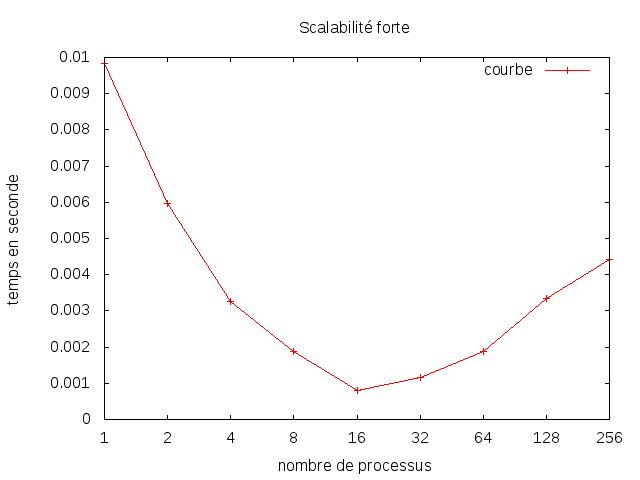
\includegraphics[height=4in]{cr/scalabilite_forte}
\caption{Scalabilité forte de Lattice Boltzman}
\end{center}
\end{figure}

\begin{figure}
\begin{center}
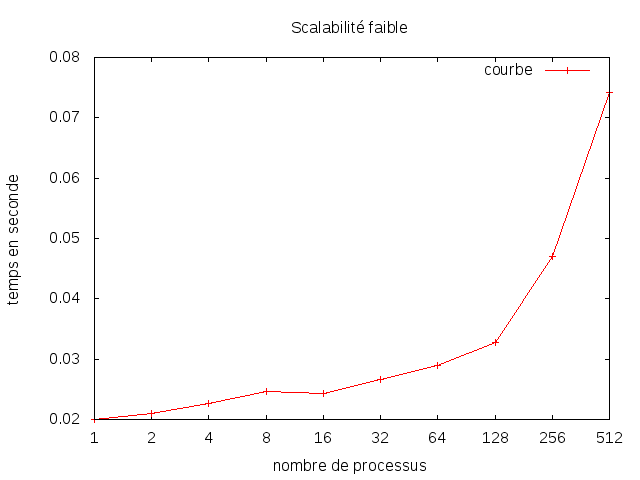
\includegraphics[height=4in]{cr/scalabilite_faible}
\caption{Scalabilité faible de Lattice Boltzman}
\end{center}
\end{figure}
